\documentclass[11pt,a4paper]{article}
\usepackage{graphicx}
%\def\hidesols{hide solutions} % uncomment this line to hide solutions
\usepackage{graphicx,comment,framed}
\usepackage{amsthm,amssymb,amsmath}
%\usepackage[colorlinks,linkcolor=blue,citecolor=blue]{hyperref}
\usepackage[rgb]{xcolor}
\usepackage{amssymb,amsmath}
\usepackage[colorlinks,linkcolor=blue,citecolor=blue]{hyperref}\usepackage{amsmath}
\usepackage{amsfonts}
\usepackage{amssymb}
\usepackage[usenames,dvipsnames]{pstricks}
\usepackage{graphicx,subfigure,wrapfig, relsize}
\usepackage{geometry,fancyhdr}
\usepackage[mathscr]{euscript}
\usepackage{multicol}
\usepackage{setspace}
\usepackage{tikz}
\usepackage{tabularx}
\usepackage{algorithmicx,algorithm}
\usepackage{mdframed}
\usepackage{xepersian}
\usepackage[noend]{algpseudocode}


%------------------------ Algorithm ------------------------------------

%\newenvironment{الگوریتم}[1]
%	{\bigskip\bigskip\begin{algorithm}\caption{#1} \label{الگوریتم: #1}\vspace{0.5em}\begin{algorithmic}[1]}
%	{\end{algorithmic}\vspace{0.5em}\end{algorithm}\bigskip}
	

%\renewcommand{\algorithmicfor}{{به ازای}}
%\renewcommand{\algorithmicwhile}{{تا وقتی}}
%\renewcommand{\algorithmicdo}{\hspace{-.2em}:}
%\renewcommand{\algorithmicif}{{اگر}}
%\renewcommand{\algorithmicthen}{\hspace{-.2em}:}
%\renewcommand{\algorithmicelse}{{در غیر این صورت:}}
%\renewcommand{\algorithmicelsif}{{در غیر این صورت اگر: }}
%\renewcommand{\algorithmicreturn}{{برگردان}}
%\renewcommand{\algorithmiccomment}[1]{$\triangleleft$ \emph{#1}}
%\renewcommand{\algorithmicrequire}{\textbf{ورودی:}}
%\renewcommand{\algorithmicensure}{\textbf{خروجی:}}

%\newcommand{\اگر}{\If}
%\newcommand{\وگرنه}{\Else}
%\newcommand{\وگر}{\ElsIf}
%\newcommand{\پایان‌اگر}{\EndIf}
%\newcommand{\به‌ازای}{\For}
%\newcommand{\پایان‌به‌ازای}{\EndFor}
%\newcommand{\تاوقتی}{\While}
%\newcommand{\پایان‌تاوقتی}{\EndWhile}
%\newcommand{\دستور}{\State}
%\newcommand{\دستورک}{\Statex}
%\newcommand{\توضیحات}{\Comment}
%\newcommand{\برگردان}{\Return}
%\renewcommand{\ورودی}{\Require}
%\newcommand{\خروجی}{\Ensure}


%--------------------- page settings ----------------------

\settextfont[Scale = 1.2 ,
             BoldFont = *Bd ,
             Extension = .ttf
            ]{XB Niloofar}
%\settextfont[Scale=1.2]{XB Niloofar}
%\setdigitfont[Scale=1.2]{XB Niloofar}
\defpersianfont\sayeh[Scale=1.2]{XB KayhanPook.ttf}
\addtolength{\textheight}{3.2cm}
\addtolength{\topmargin}{-22mm}
\addtolength{\textwidth}{2.7cm}
\addtolength{\oddsidemargin}{-1.5cm}


%------------------------ Environments ------------------------------------

\newtheorem{قضیه}{قضیه}
\newtheorem{لم}{لم}
\newtheorem{مشاهده}{مشاهده}
\newtheorem{تعریف}{تعریف}


%-------------------------- Notations ------------------------------------

\newcommand{\IR}{\ensuremath{\mathbb{R}}} 
\newcommand{\IZ}{\ensuremath{\mathbb{Z}}} 
\newcommand{\IN}{\ensuremath{\mathbb{N}}} 
\newcommand{\IS}{\ensuremath{\mathbb{S}}} 
\newcommand{\IC}{\ensuremath{\mathbb{C}}} 
\newcommand{\IB}{\ensuremath{\mathbb{B}}} 

\newcommand{\bR}{\mathbb{R}}
\newcommand{\cB}{\mathcal{B}}
\newcommand{\cO}{\mathcal{O}}
\newcommand{\cG}{\mathcal{G}}
\newcommand{\rM}{\mathrm{M}}
\newcommand{\rC}{\mathrm{C}}
\newcommand{\rV}{\mathrm{V}}

\newcommand{\lee}{\leqslant}
\newcommand{\gee}{\geqslant}
\newcommand{\ceil}[1]{{\left\lceil{#1}\right\rceil}}
\newcommand{\floor}[1]{{\left\lfloor{#1}\right\rfloor}}
\newcommand{\prob}[1]{{\mbox{\tt Pr}[#1]}}
\newcommand{\set}[1]{{\{ #1 \}}}
\newcommand{\seq}[1]{{\left< #1 \right>}}
\newcommand{\provided}{\,|\,}
\newcommand{\poly}{\mbox{\rm poly}}
\newcommand{\polylog}{\mbox{\rm \scriptsize polylog}\,}
\newcommand{\comb}[2] {\left(\!\!\begin{array}{c}{#1}\\{#2}\end{array}\!\!\right)}

\newcommand{\REM}[1]{}
\newcommand{\mrbox}[1]{\mbox{\lr{#1}}}


\newcounter{probcnt}
\newcommand{\مسئله}[1]{\stepcounter{probcnt}\bigskip\bigskip{
 	\large \bf مسئله‌ی \arabic{probcnt}$\mbox{\bf{.}}$ \ #1} \bigskip}

\newcommand{\fqed}[1]{\leavevmode\unskip\nobreak\quad\hspace*{\fill}{\ensuremath{#1}}}

\newenvironment{اثبات}
	{\begin{trivlist}\item[\hskip\labelsep{\em اثبات.}]}
	{\fqed{\square}\end{trivlist}}

\newenvironment{حل}
	{\begin{trivlist}\item[\hskip\labelsep{\bf حل.}]}
	{\fqed{\blacktriangleright}\end{trivlist}}

\ifdefined\hidesols
	\newsavebox{\trashcan} % uncomment the following line to hide solutions
	\renewenvironment{حل}{\begin{latin}\begin{lrbox}{\trashcan}}{\end{lrbox}\end{latin}}
\fi


%------------------------- Header -----------------------------

\newcommand{\سربرگ}[3]{
\parindent=0em

\rightline{
\makebox[6em][c]{

\includegraphics[height=1.6cm]{../commons/sharif.png}
}}
\vspace{-.2em}
{\scriptsize\bf دانشکده‌ی مهندسی کامپیوتر}
\hfill {\small
مدرس: مسعود صدیقین \ 
}\\[-5em]
\leftline{\hfill\Large\bf 
نظریه‌ی الگوریتمی‌ بازی‌ها
}\\[.7em]
\leftline{\hfill\bf 
نیم‌سال دوم ۰۳ -۰۲
}\\[0.7em]
\hrule height .12em

\normalsize
\vspace{1mm} #1
\hfill \small  #3
\vspace{1mm} 
\hrule height .1em

\vspace{-1.5em} 
\hfill {\sayeh\large #2} \hfill
}

% ------------------------------ Sample Input/Output --------------------------


% Bases on: https://github.com/admp/LIO-LaTeX/tree/master/other/neerc-acm

\def\s@tm@cr@s{%
\def\widthin##1{\exmpwidinf=##1\relax}\def\widthout##1{\exmpwidouf=##1\relax}%
\def\stretchin##1{\advance\exmpwidinf by ##1\relax}%
\def\stretchout##1{\advance\exmpwidouf by ##1\relax}%
}%

\newenvironment{example*}[3][]{%
\s@tm@cr@s\ttfamily\obeylines\obeyspaces\frenchspacing%\testst@r#1%
\newcommand{\exmp}[2]{%
\begin{minipage}[t]{#2}\rightskip=0pt plus 1fill\relax##1\medskip\end{minipage}&%
\begin{minipage}[t]{#3}\rightskip=0pt plus 1fill\relax##2\medskip\end{minipage}\\%
\hline}%
\begin{tabular}{|l|l|}
\hline
\multicolumn{1}{|c|}{\bf\rl{ورودی نمونه}}&%
\multicolumn{1}{|c|}{\bf\rl{خروجی نمونه}}\\%
\hline
}
{\end{tabular}}

\newenvironment{example}
	{\begin{example*}{.47\textwidth}{.475\textwidth}}
	{\end{example*}}

% ------------------------------ Table Settings --------------------------

\newcolumntype{Y}{>{\centering\arraybackslash}X}

\definecolor{lightgreen}{rgb}{0.95, 0.99, 0.97}

\newmdenv[
	topline=false,
	bottomline=false,
	skipabove=\topsep,
	skipbelow=\topsep,
	backgroundcolor=lightgreen,
	innerleftmargin=10pt,
	innerrightmargin=10pt,
	innertopmargin=10pt,
	innerbottommargin=10pt,
	leftmargin=10pt,
	rightmargin=10pt,
	leftline=false,
	rightline=false,
	linewidth=1pt
]{siderules}
	
\newenvironment{examplebox}[0]
	{\begin{siderules}\par\nobreak}
	{\end{siderules}}
	  


\begin{document}
\setstretch{1.5}

\سربرگ{تمرین دوم}{مفاهیم اولیه -  استراتژی غالب}{مهلت تحویل : -}


\مسئله{استراتژی غالب}

\textbf{الف)}
آیا اگر فردی در یک بازی چند استراتژی غالب داشته باشد، انتخاب هر کدام از این استراتژی‌ها برای او تفاوتی دارد؟ 

\textbf{ب)}
یک بازیکن حداکثر چند استراتژی غالب اکید می‌تواند داشته باشد؟

\textbf{ج)}
یک بازی مثال بزنید که در آن تنها یک بازیکن استراتژی غالب داشته باشد. 

\vspace{0.5em}
\textcolor{red}{(متین عارف‌نیا)}


\مسئله{استراتژی غالب دو}

شکل زیر یک بازی سه نفره را نشان می‌دهد. تعیین کنید آیا در این بازی، یک پروفایل استراتژی غالب یا پروفایل استراتژی غالب اکید وجود دارد یا خیر.

	{\begin{center}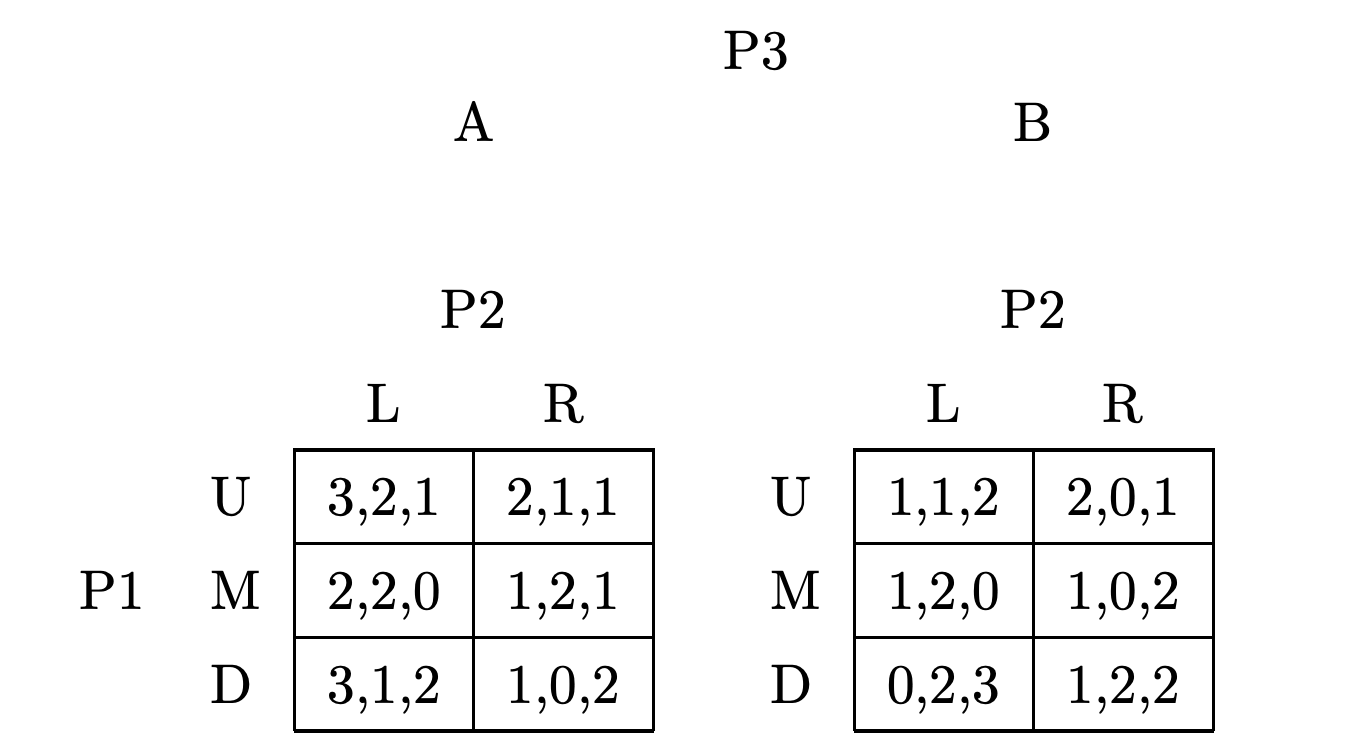
\includegraphics[width=0.5\linewidth]{pics/DSE}\end{center}}

\vspace{0.5em}
\textcolor{red}{(تحویلی - مهلت تحویل: ۲۸ بهمن ۱۴۰۲)}



\مسئله{رابطه بین پارامترها}

رابطه بین پارامترهای $a,b,c,d,e,f,g,h$ چگونه باشد که 
بازی یک معمای زندانی‌ها باشد.

\begin{latin}
	\begin{center}
		\begin{tabular}{ r|c|c| }
			\multicolumn{1}{r}{}
			&  \multicolumn{1}{c}{A}
			& \multicolumn{1}{c}{B} \\
			\cline{2-3}
			A & $a,b$ & $c,d$ \\
			\cline{2-3}
			B & $e,f$ & $g,h$ \\
			\cline{2-3}
		\end{tabular}
	\end{center}
\end{latin}
\vspace{-1.5em}
\textcolor{red}{(متین عارف‌نیا)}

\pagebreak

\مسئله{دنباله استدلال}

  مثال زیر را در نظر بگیرید.
	\begin{center}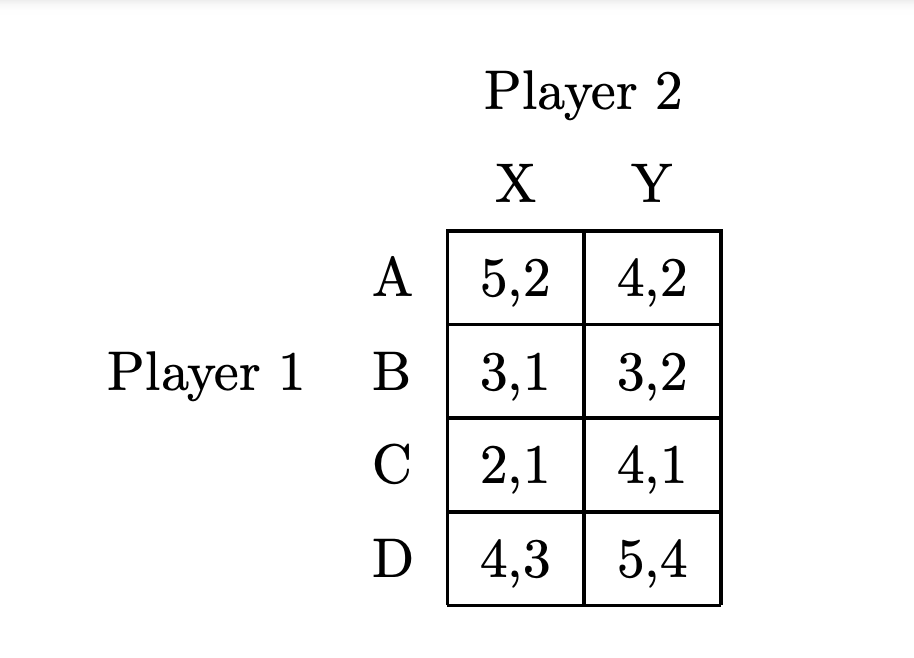
\includegraphics[width=0.3\linewidth]{pics/DSE2}\end{center}
	\textbf{الف)} 
آیا در این بازی استراتژی غالب برای هر بازیکن وجود دارد؟

	\textbf{ب)} 
	چرا بازی $B$ یا $C$ برای بازیکن سطری معقول نیست؟
	
\textbf{ج)} 
آیا می‌توان استدلال‌های قسمت‌های قبل را گسترش داد؟ به نظر شما بازی در کدام نقطه تمام می‌شود؟

\vspace{0.5em}
\textcolor{red}{(متین عارف‌نیا)}

\مسئله{دنباله استدلال ۲}

آیا می‌توانید مشابه بازی قبلی با استفاده از دنباله استدلال‌ها مشخص کنید انتظار دارید بازی در کدام نقطه تمام شود؟
	\begin{center}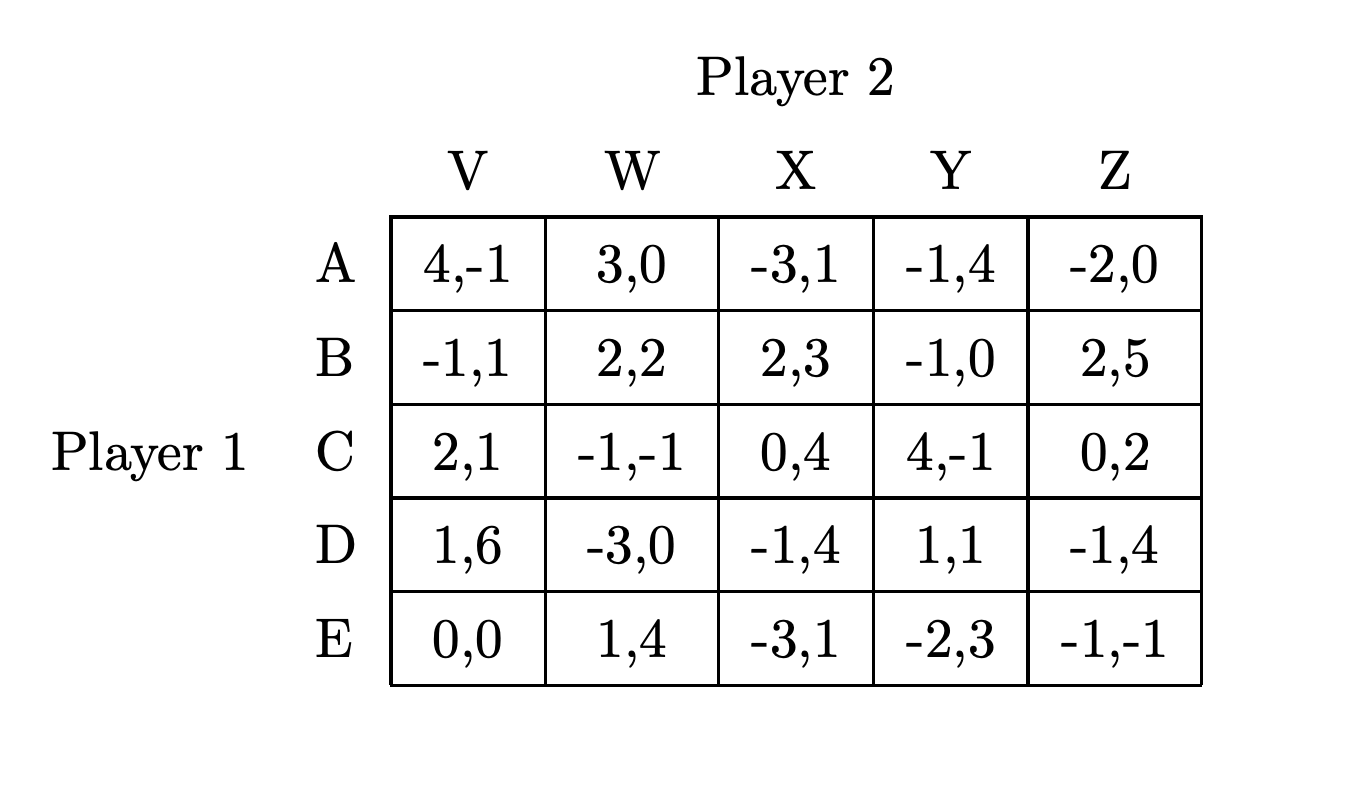
\includegraphics[width=0.4\linewidth]{pics/DSE3}\end{center}
 
\vspace{0.5em}
\textcolor{red}{(متین عارف‌نیا)}



\مسئله{حراج}

فرض کنید یک کالا قرار است حراج شود. $n$ بازیکن داریم. کالا برای بازیکن $i$ یک ارزش $w_i$ دارد که این مقدار را تنها خود بازیکن می‌داند. در حراجی، هر بازیکن یک قیمت بر روی کاغذ نوشته و تحویل می‌دهد. سپس ما بر اساس قیمت‌ها تعیین می‌کنیم که کالا به چه قیمتی و به چه کسی برسد. اگر کالا با قیمت $p$ به بازیکن $i$ برسد، سود او برابر با $w_i - p$ خواهد بود و در غیر این صورت صفر خواهد بود. در هر کدام از روش‌های حراجی زیر، مشخص کنید آیا بازیکنان استراتژی غالب دارند یا خیر.

\begin{itemize}
	\item کالا به فرد با بالاترین پیشنهاد و به قیمت  بالاترین پیشنهاد برسد.
	\item کالا به فرد با بالاترین پیشنهاد و به قیمت دومین بالاترین پیشنهاد برسد.
	\item کالا به بالاترین پیشنهاد و به قیمت سومین بالاترین پیشنهاد برسد.  
\end{itemize}

\vspace{0.5em}
\textcolor{red}{(متین عارف‌نیا)}

\مسئله{بستنی فروشی}

یک خیابان را در نظر بگیرید که به صورت بازه $[0,1000]$ مدل شده است. در نقاطی از این بازه، تعدادی خانه وجود دارد (مثلا ممکن است در نقطه $36.5$ یک خانه باشد - خانه‌ها طول و عرض ندارند، به صورت نقطه مدل می‌شوند، و در هر خانه یک نفر ساکن است). دو بستنی‌فروش، می‌خواهند هر کدام مستقلا برای محل احداث بستنی‌فروشی تصمیم بگیرند. بعد از احداث بستنی‌فروشی‌ها، ساکن هر خانه به نزدیک‌ترین بستنی‌فروشی می‌رود و یک بستنی می‌خرد. سود هر بستنی  برابر با $15000$ تومان است. مشخص کنید آیا در این بازی استراتژی غالب اکید وجود دارد؟ و اگر دارد کجاست؟

\vspace{0.5em}
\textcolor{red}{(متین عارف‌نیا)}


\مسئله{تلاش}

در یک کلاس $n$ دانش‌آموز وجود دارند.  به طور همزمان، هر دانش‌آموز $i$ یک سطح تلاش $x_i$ برای خود انتخاب می‌کند که برای او هزینه $cx_i^2$ دارد که در آن $c>0$ یک مقدار ثابت است. دانش‌آموز $i$ به خاطر تلاش‌های خود مقدار $x_i$ در نمره خود پیشرفت می‌کند؛	اما هم‌زمان این باعث می‌شود استاد کم‌تر نمودار بزند و بنابراین میزان نمره بقیه افراد به اندازه $\alpha x_i$ کاهش می‌یابد که در آن $\alpha>0$ یک مقدار ثابت است. در نتیجه، نمره نفر $i$ ام برابر خواهد بود با:
$$
x_i - \alpha \sum_{j \neq i}x_j - cx_i^2.
$$
همه اطلاعات بالا در دسترس عموم است.

	\textbf{الف)} 
	آیا این بازی یک استراتژی پروفایل غالب دارد؟
	
	
	\textbf{ب)} 
یک پروفایل $[x_1,x_2,\ldots,x_n]$ از تلاش‌ها را تعیین کنید که جمع نمرات همه دانشجویان را بیشینه می‌کند. این پروفایل را با پروفایل بخش قبل مقایسه کنید. 

\vspace{0.5em}
\textcolor{red}{(متین عارف‌نیا)}

\مسئله{تخصیص خانه}

آلیس، باب، و کارولین در حال نقل مکان به یک آپارتمان 3 خوابه (با اتاق هایی به نام های ۱، ۲، و ۳) هستند. در این مسئله ما می‌خواهیم به آن‌ها کمک کنیم اتاق‌های خود را انتخاب کنند. هر کدام از این سه نفر یک لیست ترجیح برای این سه اتاق دارد که نشان می‌دهد کدام اتاق انتخاب اول او، کدام انتخاب دوم، و کدام انتخاب سوم اوست.
این افراد به طور هم‌زمان ترجیحات خود را در یک پاکت ارسال می‌کنند و سپس اتاق‌‌ها بر اساس یکی از مکانیزم‌های زیر اختصاص داده می‌شوند. برای هر مکانیزم، بررسی کنید که آیا ارسال ترجیحات واقعی یک استراتژی غالب است یا خیر؟

 	\textbf{الف)} 
 	ابتدا به آلیس، گزینه اولش را اختصاص می‌دهیم. سپس باب از بین اتاق‌های باقی‌مانده بهترین انتخابش را می‌گیرد و در نهایت اتاق باقی‌مانده به کارولین می‌رسد.
 	

	 	\textbf{ب)}
	 	ابتدا آلیس و باب را مقایسه می‌کنیم. اگر انتخاب اول هر دو متفاوت بود، به هر دوی آن‌ها انتخاب اولشان را می‌دهیم و خانه باقی‌مانده به کارولین می‌رسد. در غیر این صورت، همین کار را با آلیس و کارولین انجام می‌دهیم. نهایتا، اگر انتخاب اول همه یکی بود، از الگوریتم بخش اول برای تخصیص استفاده می‌کنیم.

\vspace{0.5em}
\textcolor{red}{(متین عارف‌نیا)}
\end{document}
